\section{Architecture Overview}
\label{sec:overview}

The overview of the rule-based solution is illustrated in \figref{fig:overview}. The input of the transformation is a \emph{movie model}. The result is a \emph{transformed movie model} containing additional model elements, including various groups (couples and $n$-cliques) and their average rating~\cite{Horn14}. The transformation runs in a Java application, that uses \emph{pattern matchers} provided by \incquery{} and model modification code specified in Xtend.
The model \emph{modifications} are performed over EMF resources, while the pattern matcher \emph{monitors} the resources to incrementally update match sets.
The application initially reads the input movie database resource, creates the output resources (organizing them into a resource set), then executes the transformation, and finally serializes the results into files.

\begin{figure}
	\centering
	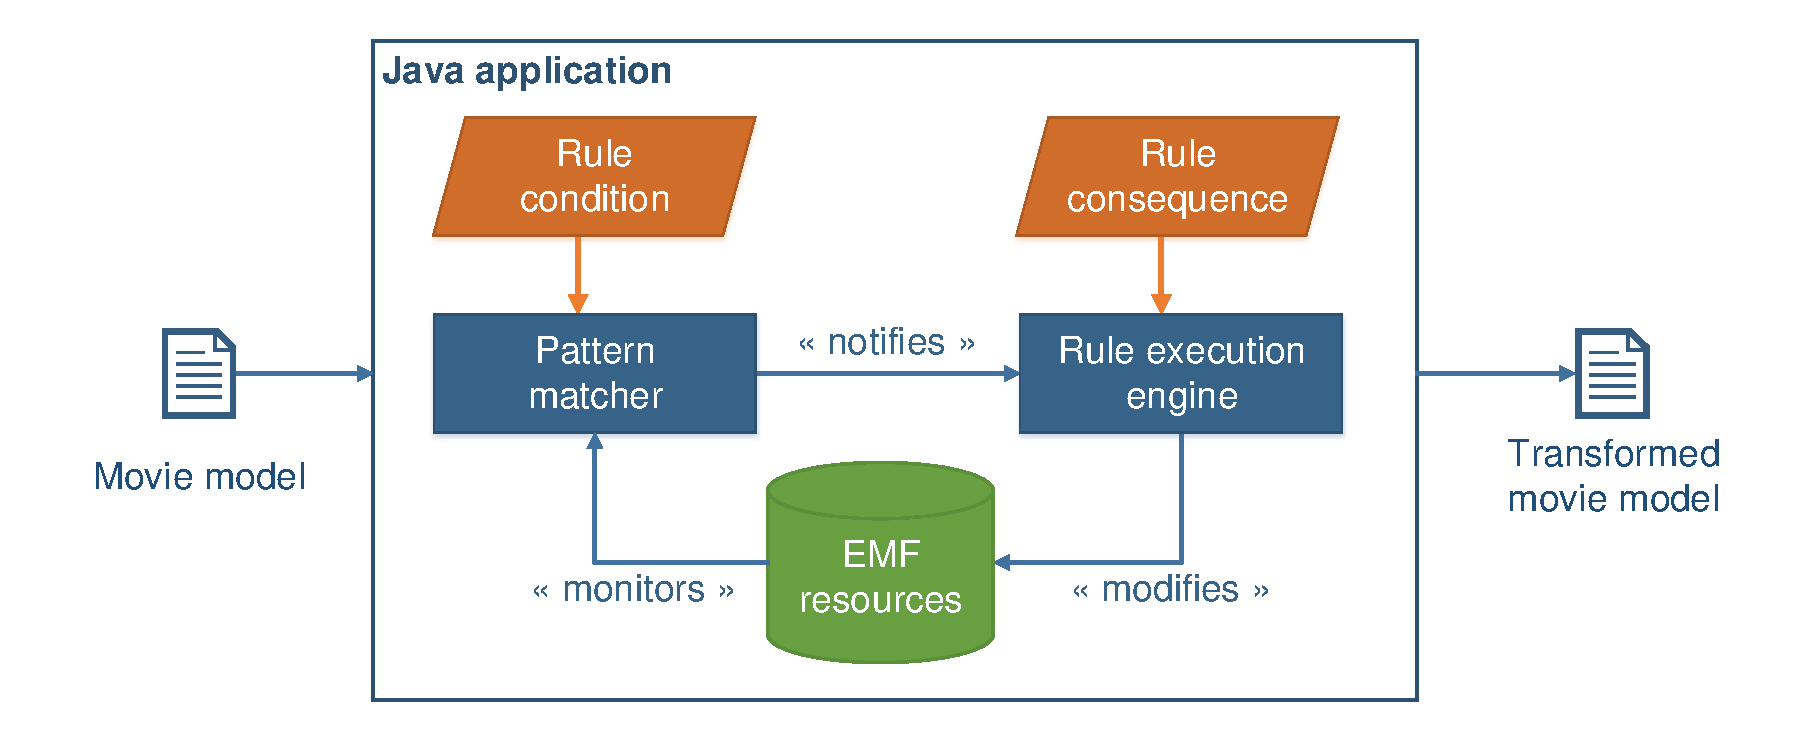
\includegraphics[width=.9\textwidth]{architecture.pdf}
	\caption{Overview of the specification and runtime.}\label{fig:overview}
\end{figure}

The whole solution is implemented in two languages. Rule conditions are formulated as \incquery{} graph patterns, while the rule consequences (model manipulations) in Xtend. Since the advanced transformation constructs of \incquery{} are tailored for event-driven (incremental) execution, the current solution only uses pattern matchers to access query results, without additional constructs.